% !TeX root = ../main.tex
\section{Khám phá và tiền xử lý dữ liệu}\label{sec:eda}

Khám phá dữ liệu (Exploratory Data Analysis, EDA) được làm trước khi thiết kế kho dữ liệu, để biết dữ liệu thiếu ở đâu, sai ở đâu, phân bố ra sao; mỗi quy tắc làm sạch về sau đều dựa trên kết quả này \cite{han}. Phần này gồm ba bước: khám phá dữ liệu thô, đặt quy tắc tiền xử lý, rồi khám phá lại dữ liệu sau xử lý.

Phần khám phá dữ liệu thô được chạy trực tiếp trên chín tập tin CSV bằng chương trình \code{src/eda/run\_eda.py}, độc lập với quy trình ETL, nên các con số ở đây cũng là căn cứ để đối soát kết quả ETL ở mục~\ref{sec:hienthuc}. Phần khám phá sau tiền xử lý đọc từ các bảng đã làm sạch trong staging và từ Data Mart.

\subsection{Khám phá dữ liệu thô}\label{sec:edatho}

\subsubsection{Cấu trúc các tập dữ liệu}

Bảng~\ref{tab:cautruc} tóm tắt cấu trúc của chín tập tin: tổng cộng 52 cột. Bốn tập \code{order\_items}, \code{order\_payments}, \code{customers} và \code{sellers} không thiếu giá trị nào và không có dòng trùng. Giá trị thiếu tập trung ở ba tập \code{orders}, \code{order\_reviews} và \code{products}; dòng trùng chỉ xuất hiện ở \code{geolocation}.

\begin{table}[H]
\centering
\small\setstretch{1.1}
\caption{Cấu trúc, giá trị thiếu và dòng trùng của các tập dữ liệu thô}
\label{tab:cautruc}
\begin{tabularx}{\linewidth}{|>{\raggedright\arraybackslash}X|P{1.8cm}|P{1.2cm}|P{1.6cm}|P{1.8cm}|P{1.5cm}|}
\hline
\textbf{Tập tin} & \textbf{Số dòng} & \textbf{Số cột} & \textbf{Ô bị thiếu} & \textbf{Dòng có ô thiếu} & \textbf{Dòng trùng}\\ \hline
\code{orders} & 99.441 & 8 & 4.908 & 2.980 & 0\\ \hline
\code{order\_items} & 112.650 & 7 & 0 & 0 & 0\\ \hline
\code{order\_payments} & 103.886 & 5 & 0 & 0 & 0\\ \hline
\code{order\_reviews} & 99.224 & 7 & 145.903 & 89.385 & 0\\ \hline
\code{customers} & 99.441 & 5 & 0 & 0 & 0\\ \hline
\code{sellers} & 3.095 & 4 & 0 & 0 & 0\\ \hline
\code{products} & 32.951 & 9 & 2.448 & 611 & 0\\ \hline
\code{geolocation} & 1.000.163 & 5 & 0 & 0 & 261.831\\ \hline
\code{category\_translation} & 71 & 2 & 0 & 0 & 0\\ \hline
\end{tabularx}
\end{table}

\subsubsection{Phân tích giá trị thiếu}

Hình~\ref{fig:giatrithieu} cho thấy tỷ lệ thiếu của 13 cột có giá trị thiếu (các cột thiếu ở cùng những dòng được gộp lại). Hai cột thiếu nhiều nhất là tiêu đề và nội dung bình luận đánh giá, lần lượt 88,3\% và 58,7\%. Đây không phải lỗi: khách chỉ chấm sao mà không viết gì là chuyện bình thường. Tuy vậy, 26,6\% bình luận có nội dung đi kèm điểm 1-2 sao, trong khi con số này ở các đánh giá không có nội dung chỉ là 6,3\%; nghĩa là khách thường viết khi không hài lòng.

\begin{figure}[H]
\centering
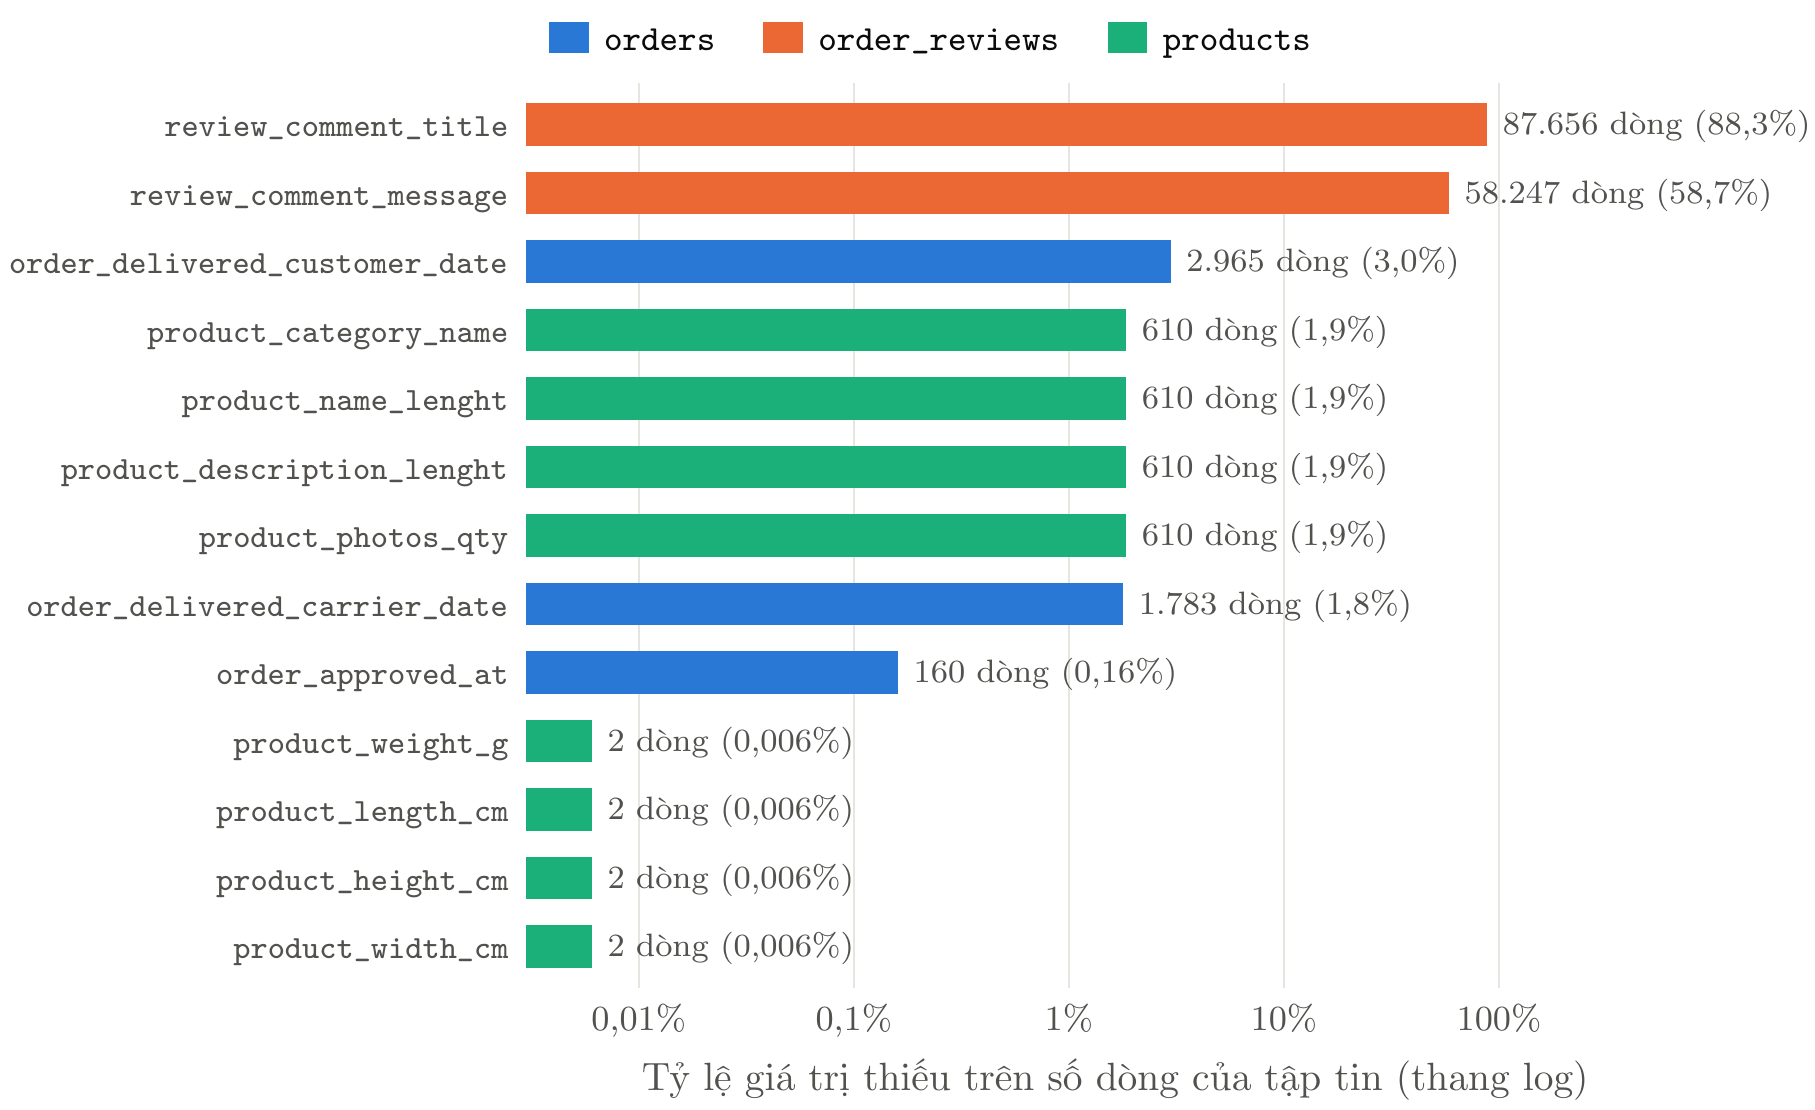
\includegraphics{Pictures/fig-eda-gia-tri-thieu.png}
\caption{Số dòng và tỷ lệ giá trị thiếu theo cột trong dữ liệu thô (trục ngang theo thang log)}
\label{fig:giatrithieu}
\end{figure}

Ba cột mốc thời gian của \code{orders} thiếu ít hơn nhiều, và phần lớn có lý do nghiệp vụ. Trong 2.965 đơn thiếu ngày nhận hàng, 2.957 đơn chưa từng được giao (đang vận chuyển, bị hủy hoặc hết hàng); chỉ 8 đơn ở trạng thái \code{delivered} mà không có ngày nhận. Tương tự, 1.781 trên 1.783 đơn thiếu ngày bàn giao vận chuyển là đơn chưa được bàn giao, và 141 trên 160 đơn thiếu thời điểm duyệt là đơn bị hủy. Vì vậy, điền giá trị thay thế (như trung bình) cho các cột này là sai: một đơn bị hủy không có ngày giao hàng nào cả. Ở tập \code{products}, 610 sản phẩm thiếu cùng lúc ngành hàng và ba cột mô tả, còn 2 sản phẩm thiếu cùng lúc khối lượng và ba cột kích thước; đây là những sản phẩm được đăng thiếu thông tin chứ không phải lỗi rải rác.

\subsubsection{Phát hiện giá trị ngoại lai}

Ngoại lai của bốn thước đo số chính được xác định bằng quy tắc khoảng tứ phân vị (IQR): một giá trị là ngoại lai nếu lớn hơn $Q_3 + 1{,}5 \times (Q_3 - Q_1)$ \cite{han}. Hình~\ref{fig:ngoailai} cho thấy cả bốn thước đo đều lệch phải mạnh. Ví dụ, giá bán có trung vị 74,99 BRL nhưng 8.427 dòng (7,5\%) vượt ngưỡng 277,40 BRL, cao nhất là 6.735 BRL; thời gian giao hàng có trung vị 10,2 ngày, 4.899 đơn (5,1\%) vượt ngưỡng 29,2 ngày, lâu nhất là 209,6 ngày.

\begin{figure}[H]
\centering
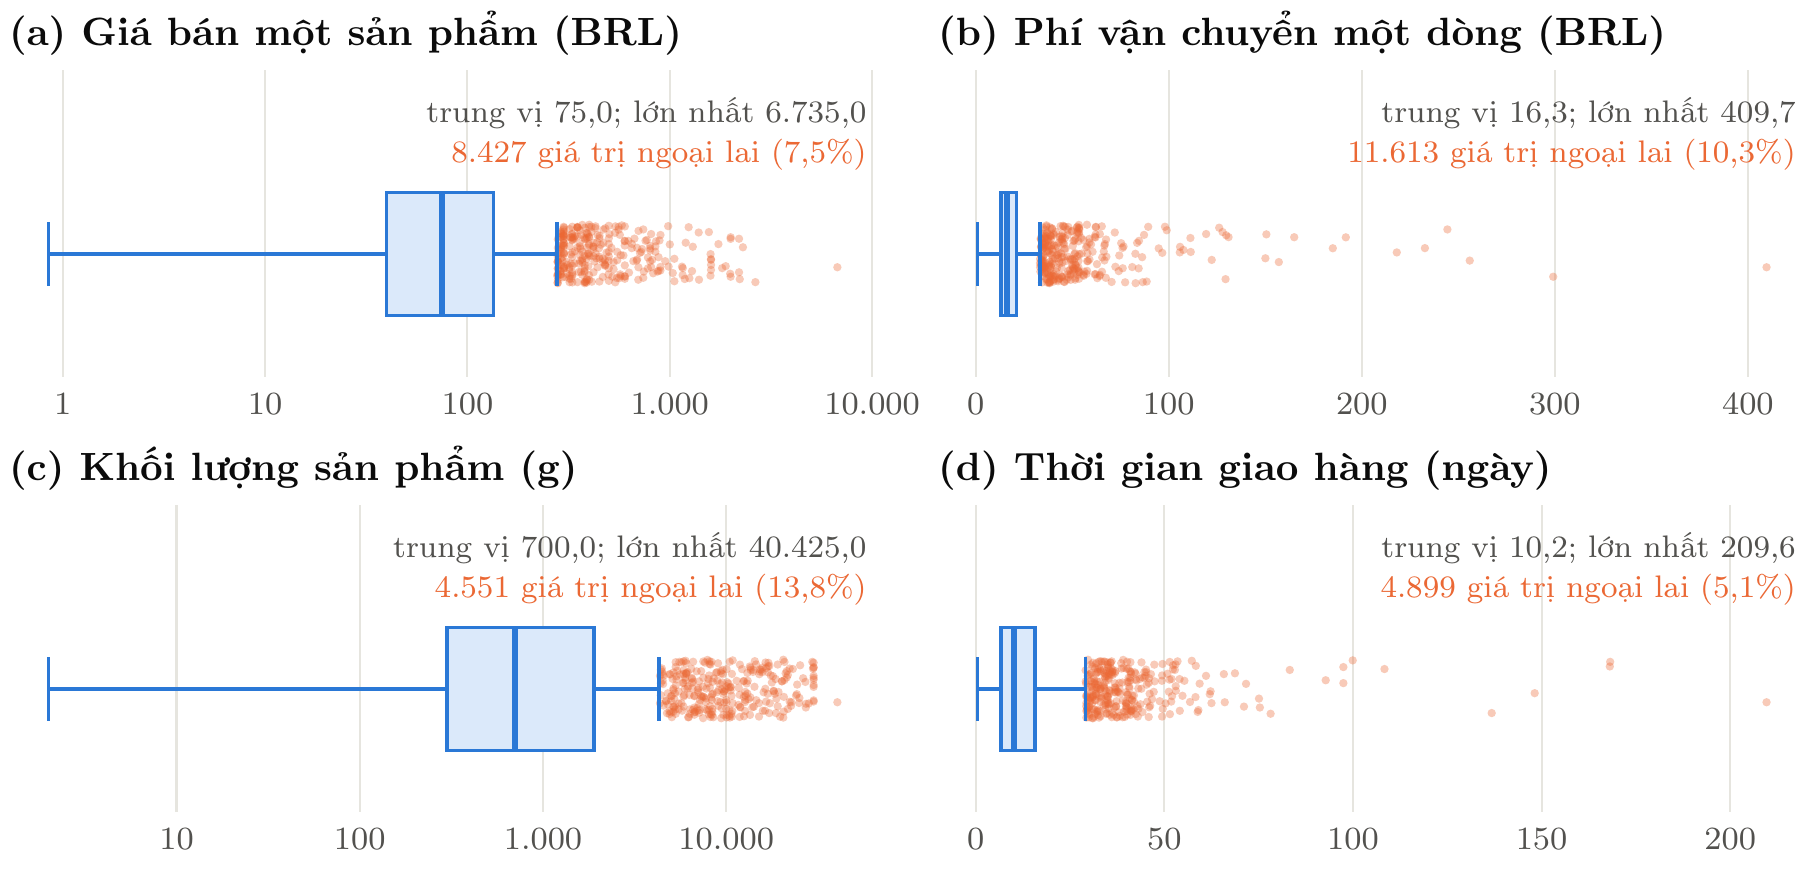
\includegraphics{Pictures/fig-eda-ngoai-lai.png}
\caption{Phân bố và giá trị ngoại lai (theo quy tắc IQR) của bốn thước đo số; điểm cam là một mẫu 300 giá trị ngoại lai, số đếm tính trên toàn bộ dữ liệu}
\label{fig:ngoailai}
\end{figure}

Các giá trị ngoại lai này được \textit{giữ lại}. Một sản phẩm giá vài nghìn BRL hay nặng vài chục ki-lô-gam là giao dịch thật, không phải lỗi nhập liệu; cắt bớt sẽ làm sai tổng doanh thu, mà tổng doanh thu phải khớp với nguồn ở bước đối soát. Các giá trị thật sự vô lý chỉ có hai nhóm nhỏ: 4 sản phẩm có khối lượng bằng 0 và các mốc thời gian sai thứ tự, được xử lý riêng ở Bảng~\ref{tab:quytac}. Do phân bố lệch, khi so sánh giữa các nhóm, báo cáo luôn xem trung vị hoặc tỷ lệ chứ không chỉ trung bình. Phí vận chuyển bằng 0 (383 dòng) cũng được giữ, vì đó là các đơn được miễn phí vận chuyển.

\subsubsection{Phân bố thời gian giao hàng và điểm đánh giá}

Với 96.470 đơn đã giao có đủ ngày nhận hàng, thời gian giao trung bình là 12,6 ngày nhưng trung vị chỉ 10,2 ngày (Hình~\ref{fig:thoigiangiao}a). Phần lớn đơn đến tay khách trong vòng hai tuần, nhưng có 4,7\% đơn mất hơn 30 ngày. Hình~\ref{fig:thoigiangiao}b so sánh ngày nhận hàng thực tế với ngày giao dự kiến mà sàn hứa với khách. Trung vị là 12 ngày \textit{trước} hạn, và 78,9\% đơn về sớm từ một tuần trở lên. Nói cách khác, sàn đặt ngày dự kiến khá rộng, nên phần lớn đơn đều đúng hạn. Chỉ 6,77\% đơn bị trễ, nhưng như sẽ thấy ở phần OLAP, nhóm đơn này ảnh hưởng rất mạnh đến điểm đánh giá.

\begin{figure}[H]
\centering
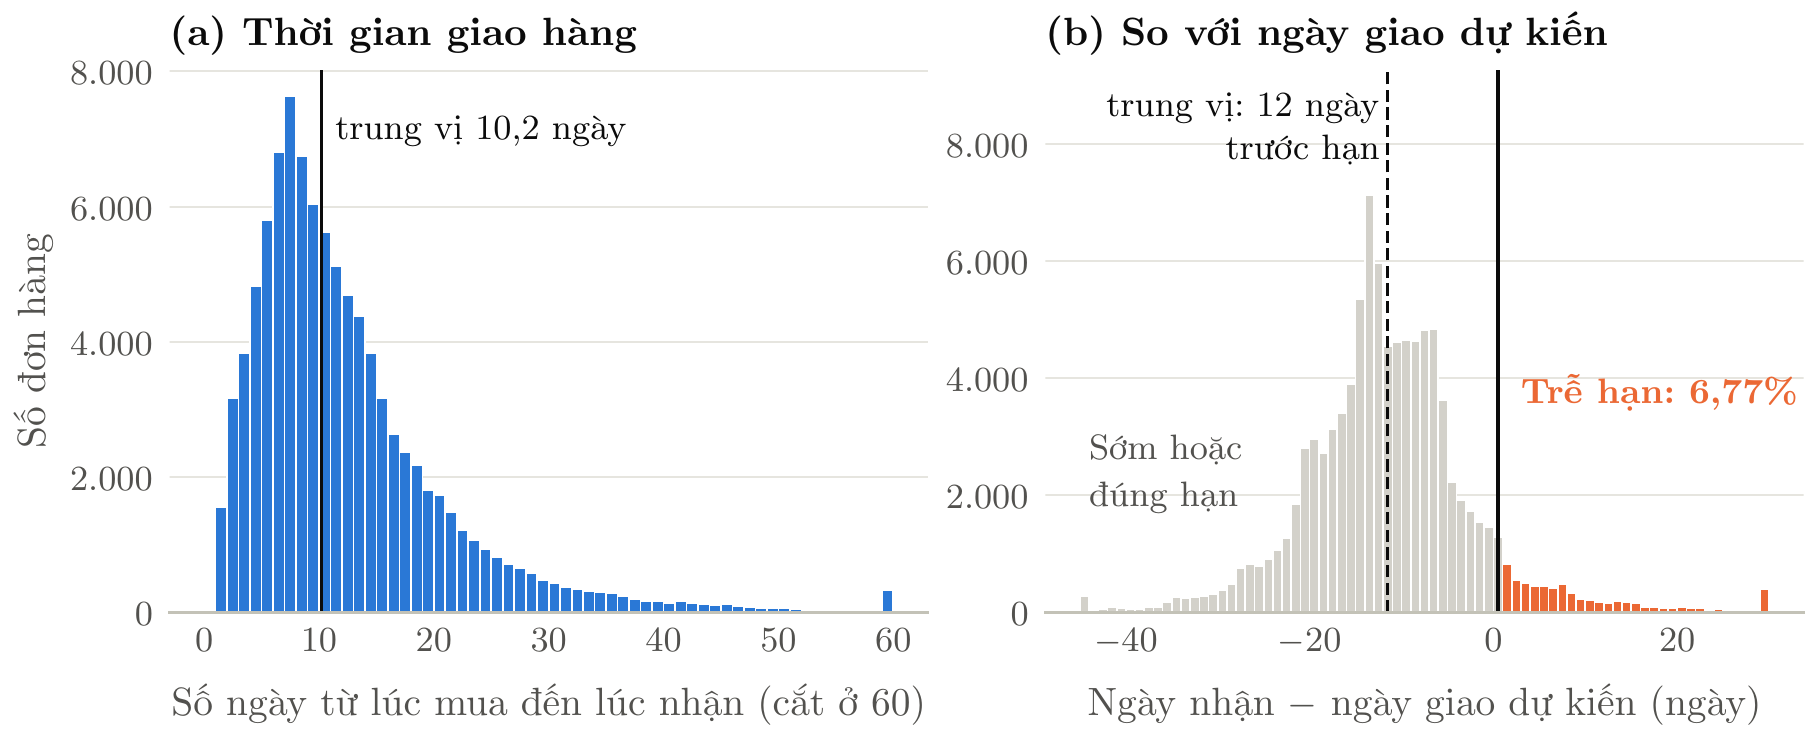
\includegraphics{Pictures/fig-thoi-gian-giao-hang.png}
\caption{Phân bố thời gian giao hàng (a) và chênh lệch giữa ngày nhận hàng với ngày giao dự kiến (b); màu cam là các đơn giao trễ}
\label{fig:thoigiangiao}
\end{figure}

Về đánh giá, sau khi giữ một đánh giá cho mỗi đơn hàng (cách chọn ở Bảng~\ref{tab:quytac}), có 98.673 đánh giá. Điểm phân cực rõ (Hình~\ref{fig:danhgia}): 57,8\% đánh giá là 5 sao, nhưng 1 sao lại chiếm 11,5\%, nhiều hơn cả 2 sao và 3 sao cộng lại. Điều này gợi ý rằng khách hàng thường chỉ chấm điểm thấp khi gặp một sự cố cụ thể, và giao trễ là ứng viên đầu tiên cần kiểm tra.

\begin{figure}[H]
\centering
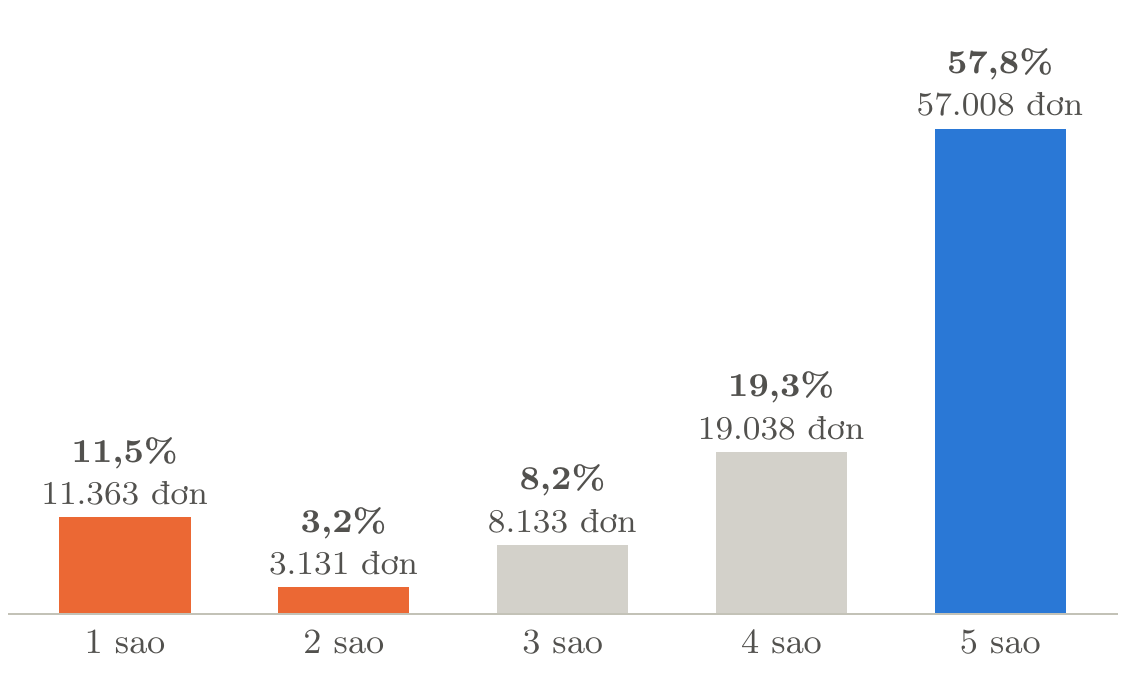
\includegraphics{Pictures/fig-phan-bo-danh-gia.png}
\caption{Phân bố điểm đánh giá của 98.673 đơn hàng (mỗi đơn một đánh giá)}
\label{fig:danhgia}
\end{figure}

\subsubsection{Tổng hợp các vấn đề chất lượng dữ liệu}

Ngoài giá trị thiếu và ngoại lai, dữ liệu còn được kiểm tra về tính duy nhất của khóa, thứ tự các mốc thời gian, tính nhất quán giữa các tập và cách viết tên địa danh. Bảng~\ref{tab:chatluong} liệt kê toàn bộ 31 vấn đề tìm được; đây là đầu vào trực tiếp cho bước tiền xử lý ở mục~\ref{sec:tienxuly}.

\begingroup\small\setstretch{1.1}
\begin{longtable}{|p{3.3cm}|p{8.2cm}|p{2.6cm}|}
\caption{Các vấn đề về chất lượng dữ liệu nguồn}\label{tab:chatluong}\\
\hline
\textbf{Tập dữ liệu} & \textbf{Vấn đề phát hiện} & \textbf{Số lượng}\\ \hline \endfirsthead
\hline
\textbf{Tập dữ liệu} & \textbf{Vấn đề phát hiện} & \textbf{Số lượng}\\ \hline \endhead
\code{orders} & Thiếu thời điểm duyệt đơn & 160 đơn\\ \hline
\code{orders} & Thiếu thời điểm bàn giao vận chuyển & 1.783 đơn\\ \hline
\code{orders} & Thiếu thời điểm khách nhận hàng & 2.965 đơn\\ \hline
\code{orders} & Trạng thái đã giao nhưng thiếu thời điểm nhận hàng & 8 đơn\\ \hline
\code{orders} & Thời điểm bàn giao vận chuyển sau thời điểm khách nhận hàng & 23 đơn\\ \hline
\code{orders} & Thời điểm bàn giao vận chuyển trước thời điểm duyệt đơn & 1.359 đơn\\ \hline
\code{orders} & Đơn hàng không có dòng sản phẩm & 775 đơn\\ \hline
\code{orders} & Đơn hàng không có dữ liệu thanh toán & 1 đơn\\ \hline
\code{orders} & Đơn hàng không có đánh giá & 768 đơn\\ \hline
\code{orders} & Giai đoạn đầu và cuối có rất ít dữ liệu (2016; 09-10/2018) & 349 đơn\\ \hline
\code{order\_items} & Phí vận chuyển bằng 0 & 383 dòng\\ \hline
\code{order\_payments} & Phương thức thanh toán không xác định (\code{not\_defined}) & 3 dòng\\ \hline
\code{order\_payments} & Giá trị thanh toán bằng 0 & 9 dòng\\ \hline
\code{order\_payments} & Số kỳ trả góp bằng 0 & 2 dòng\\ \hline
\code{order\_payments} & Tổng thanh toán lệch hơn 1 BRL (đồng Real Brazil) so với tiền hàng cộng phí vận chuyển & 249 đơn\\ \hline
\code{order\_reviews} & Một \code{review\_id} xuất hiện trên nhiều đơn hàng & 789 mã\\ \hline
\code{order\_reviews} & Một đơn hàng có nhiều đánh giá & 547 đơn\\ \hline
\code{order\_reviews} & Không có nội dung bình luận & 58,7\% số dòng\\ \hline
\code{order\_reviews} & Không có tiêu đề bình luận & 88,3\% số dòng\\ \hline
\code{products} & Thiếu ngành hàng và thông tin mô tả & 610 sản phẩm\\ \hline
\code{products} & Thiếu khối lượng và kích thước & 2 sản phẩm\\ \hline
\code{products} & Khối lượng bằng 0 & 4 sản phẩm\\ \hline
\code{products} & Sai chính tả tên cột (\code{product\_name\_lenght}, \code{product\_description\_lenght}) & 2 cột\\ \hline
\code{translation} & Ngành hàng chưa có bản dịch (\code{pc\_gamer} và một ngành hàng về dụng cụ nhà bếp) & 2 ngành hàng\\ \hline
\code{sellers} & Tên thành phố không chuẩn, ví dụ \code{sao paulo / sao paulo}, \code{sbc/sp}, \code{04482255} & 68 người bán\\ \hline
\code{sellers} & Mã bưu chính không có trong \code{geolocation} & 7 người bán\\ \hline
\code{customers} & Mã bưu chính không có trong \code{geolocation} & 278 khách hàng\\ \hline
\code{geolocation} & Dòng trùng lặp hoàn toàn & 261.831 dòng\\ \hline
\code{geolocation} & Tọa độ nằm ngoài lãnh thổ Brazil & 42 dòng\\ \hline
\code{geolocation} & Một mã bưu chính thuộc nhiều bang & 8 mã\\ \hline
\code{geolocation} & Một mã bưu chính ứng với nhiều cách viết tên thành phố & 8.556 mã\\ \hline
\end{longtable}
\endgroup

Các khóa chính của \code{orders} và \code{order\_items} đều toàn vẹn, nên phần lớn vấn đề nằm ở ba nhóm: giá trị thiếu, dữ liệu địa lý chưa chuẩn hóa, và mốc thời gian sai thứ tự. Dữ liệu địa lý là phần phải xử lý nhiều nhất. Khi vẽ toàn bộ tọa độ phân biệt lên mặt phẳng (Hình~\ref{fig:toado}a), 42 dòng (33 điểm phân biệt) rơi ra ngoài khung lãnh thổ Brazil, có điểm nằm ở châu Âu hoặc Bắc Mỹ. Nếu không loại các điểm này, tọa độ trung bình của thành phố sẽ bị kéo lệch hẳn. Phần còn lại (Hình~\ref{fig:toado}b) cho thấy khách hàng tập trung dày đặc ở vùng Đông Nam, quanh São Paulo và Rio de Janeiro.

\begin{figure}[H]
\centering
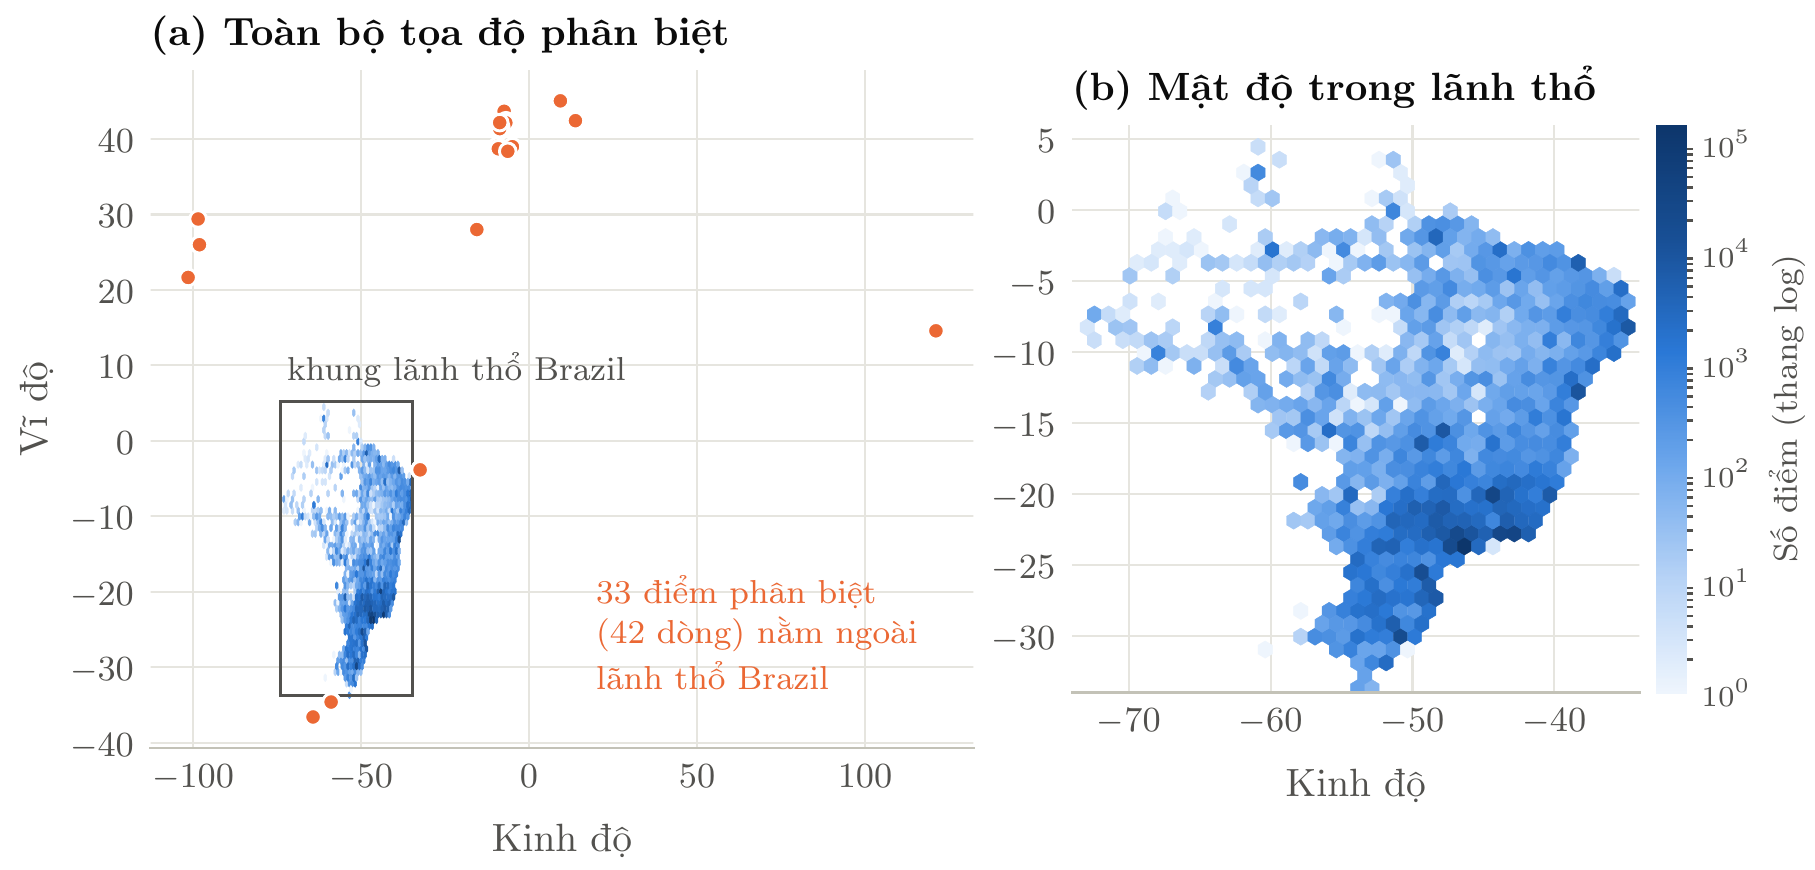
\includegraphics{Pictures/fig-toa-do-geolocation.png}
\caption{Tọa độ phân biệt trong tập \code{geolocation}: toàn bộ (a), khung chữ nhật là giới hạn lãnh thổ Brazil, và phần nằm trong lãnh thổ (b)}
\label{fig:toado}
\end{figure}
\subsection{Tiền xử lý dữ liệu}\label{sec:tienxuly}

Mỗi vấn đề ở Bảng~\ref{tab:chatluong} có một quy tắc xử lý riêng, được hiện thực ở bước transformation của quy trình ETL (mục~\ref{sec:thietke}); phần này chỉ nêu \textit{xử lý thế nào và vì sao}.

\subsubsection{Làm sạch dữ liệu}

Nguyên tắc chung là giữ lại càng nhiều dữ liệu hợp lệ càng tốt. Khi một mốc thời gian có vấn đề, chỉ thước đo liên quan bị để trống, còn đơn hàng vẫn được giữ; không có giá trị nào được điền bằng trung bình, vì như đã phân tích ở trên, phần lớn giá trị thiếu là thiếu có lý do. Bảng~\ref{tab:quytac} là quy tắc cho từng vấn đề ở Bảng~\ref{tab:chatluong}.

\begingroup\small\setstretch{1.1}
\begin{longtable}{|P{5.3cm}|P{8.6cm}|}
\caption{Quy tắc xử lý các vấn đề chất lượng dữ liệu}\label{tab:quytac}\\
\hline
\textbf{Vấn đề} & \textbf{Quy tắc xử lý}\\ \hline \endfirsthead
\hline
\textbf{Vấn đề} & \textbf{Quy tắc xử lý}\\ \hline \endhead
Đơn hàng thiếu thời điểm duyệt, bàn giao vận chuyển hoặc nhận hàng & Giữ lại đơn hàng. Cột ngày tương ứng được gán về bản ghi không xác định, các khoảng thời gian liên quan và cờ giao trễ để trống.\\ \hline
Đơn hàng đã giao nhưng thiếu thời điểm nhận hàng (8 đơn) & Giữ lại, xử lý như đơn chưa có ngày nhận hàng và không tính vào các chỉ số giao hàng.\\ \hline
Thời điểm bàn giao vận chuyển sau thời điểm nhận hàng (23 đơn) & Giữ tổng thời gian giao hàng, để trống thời gian vận chuyển vì không xác định được thứ tự đúng.\\ \hline
Thời điểm bàn giao vận chuyển trước thời điểm duyệt (1.359 đơn) & Giữ các mốc thời gian, để trống thời gian chuẩn bị hàng vì giá trị bị âm.\\ \hline
Đơn hàng không có dòng sản phẩm (775 đơn) & Không nạp vào bảng fact, ghi nhận vào nhật ký ETL.\\ \hline
Đơn hàng không có đánh giá (768 đơn) & Điểm đánh giá để trống, ngày đánh giá gán về bản ghi không xác định.\\ \hline
Đơn hàng có nhiều đánh giá (547 đơn) & Chọn đánh giá có thời điểm phản hồi muộn nhất làm đánh giá chính thức của đơn hàng, vì có 202 đơn trong số này có các điểm đánh giá khác nhau.\\ \hline
Một \code{review\_id} xuất hiện trên nhiều đơn hàng (789 mã) & Không xử lý riêng, vì đánh giá được gắn vào bảng fact theo \code{order\_id}.\\ \hline
Giá trị ngoại lai của giá, phí vận chuyển, khối lượng, thời gian giao & Giữ nguyên vì là giao dịch thật; phí vận chuyển bằng 0 (383 dòng) xem là miễn phí vận chuyển.\\ \hline
Sản phẩm thiếu ngành hàng (610 sản phẩm) & Gán vào ngành hàng ``không xác định''.\\ \hline
Sản phẩm thiếu hoặc có khối lượng, kích thước bằng 0 (6 sản phẩm) & Để trống các thuộc tính này.\\ \hline
Ngành hàng chưa có bản dịch (2 ngành hàng) & Bổ sung tên tiếng Anh thủ công vào bảng ngành hàng.\\ \hline
Tên thành phố của người bán không chuẩn & Chuyển về chữ thường, bỏ dấu, bỏ phần mã bang thừa như ``/ sp'' hoặc ``- sp''. Nếu tên sau chuẩn hóa không có trong \code{geolocation} của bang tương ứng (ví dụ tên là chuỗi số, tên viết tắt hoặc viết sai chính tả) thì lấy tên thành phố theo mã bưu chính.\\ \hline
Dòng trùng lặp trong \code{geolocation} (261.831 dòng) & Loại bỏ, chỉ giữ lại 738.332 dòng phân biệt.\\ \hline
Tọa độ nằm ngoài lãnh thổ Brazil (42 dòng) & Loại bỏ trước khi tính tọa độ trung bình của thành phố.\\ \hline
Mã bưu chính thuộc nhiều bang (8 mã) & Chọn bang xuất hiện nhiều nhất của mã bưu chính đó.\\ \hline
Mã bưu chính không có trong \code{geolocation} (278 khách hàng, 7 người bán) & Vẫn lấy tên thành phố và bang từ bảng khách hàng hoặc người bán; tọa độ để trống.\\ \hline
Các mã thanh toán bất thường (giá trị 0, phương thức không xác định) & Không ảnh hưởng đến Data Mart vì dữ liệu thanh toán không được nạp vào bảng fact; chỉ lưu lại trong khu vực staging.\\ \hline
\end{longtable}
\endgroup

Với quy tắc chọn đánh giá: trong 547 đơn có nhiều đánh giá, 202 đơn có các điểm khác nhau, nên lấy trung bình sẽ tạo ra những điểm như 3,5 vốn không tồn tại trong thực tế. Đánh giá được phản hồi muộn nhất được giữ lại vì đó là ý kiến cuối cùng của khách về đơn hàng.

\subsubsection{Chuẩn hóa, tích hợp và tạo thuộc tính mới}

Bên cạnh làm sạch, dữ liệu cần được đưa về cùng một dạng để các tập nối được với nhau. Kiểu dữ liệu được thống nhất: thời gian sang \code{timestamp}, tiền sang số thập phân, mã bưu chính giữ dạng chuỗi để không mất số 0 ở đầu. Mỗi khách hàng thật được nhận diện bằng \code{customer\_unique\_id} thay cho \code{customer\_id} sinh theo từng đơn. Tên thành phố của khách hàng và người bán được chuẩn hóa theo cùng một quy tắc rồi gộp thành một danh sách thành phố duy nhất, có tọa độ là trung bình các điểm \code{geolocation} hợp lệ.

Một số thuộc tính mới được tạo thêm để phục vụ phân tích. Bốn khoảng thời gian (duyệt đơn, chuẩn bị hàng, vận chuyển, tổng thời gian giao) được tính từ các mốc của đơn hàng; cờ giao trễ được tính bằng cách so ngày nhận hàng với ngày giao dự kiến. 27 bang được gom thành năm vùng địa lý, và mỗi ngày được tách thành tháng, quý, năm, thứ trong tuần, giống như cách rời rạc hóa (binning) một thuộc tính liên tục thành các nhóm để phân tích theo nhiều mức. Cách tính chi tiết của từng thuộc tính nằm ở phần thiết kế ETL.

\subsubsection{Kết quả tiền xử lý}

Bảng~\ref{tab:truocsau} so sánh số lượng bản ghi trước và sau tiền xử lý. Số đơn hàng, dòng sản phẩm, khách hàng và sản phẩm không mất đi bản ghi hợp lệ nào; chênh lệch chỉ đến từ những chỗ có chủ đích: 775 đơn không có sản phẩm không vào bảng fact, mỗi đơn chỉ giữ một đánh giá, và mỗi khách hàng thật chỉ còn một dòng. Bảng \code{geolocation} giảm từ hơn một triệu dòng xuống 738.299 dòng sau khi bỏ dòng trùng và tọa độ sai. Ở người bán, 636 cách viết (thành phố, bang) khác nhau được quy về 580 thành phố thật.

\begin{table}[H]
\centering
\small\setstretch{1.1}
\caption{Số lượng bản ghi trước và sau tiền xử lý}
\label{tab:truocsau}
\begin{tabularx}{\linewidth}{|>{\raggedright\arraybackslash}X|r|r|r|}
\hline
\textbf{Đối tượng} & \textbf{Dữ liệu thô} & \textbf{Sau làm sạch} & \textbf{Trong Data Mart}\\ \hline
Đơn hàng & 99.441 & 99.441 & 98.666\\ \hline
Dòng sản phẩm trong đơn & 112.650 & 112.650 & 112.650\\ \hline
Đánh giá & 99.224 & 98.673 & 97.917\\ \hline
Khách hàng (mã theo đơn $\rightarrow$ khách hàng thật) & 99.441 & 96.096 & 96.096\\ \hline
Sản phẩm & 32.951 & 32.951 & 32.951\\ \hline
Dòng tọa độ \code{geolocation} & 1.000.163 & 738.299 & --\\ \hline
Cách viết (thành phố, bang) của người bán & 636 & 580 & 580\\ \hline
Cách viết (thành phố, bang) của khách hàng & 4.310 & 4.301 & 4.301\\ \hline
Thành phố (khách hàng và người bán) & -- & 4.341 & 4.341\\ \hline
\end{tabularx}
\end{table}

Số đánh giá trong Data Mart (97.917) ít hơn sau làm sạch (98.673) vì một số đánh giá thuộc về các đơn không có dòng sản phẩm, những đơn này không vào bảng fact.

\subsection{Khám phá dữ liệu sau tiền xử lý}\label{sec:edasach}

Sau khi làm sạch, dữ liệu được gom về mức đơn hàng (96.470 đơn đã giao) để khảo sát lại quan hệ giữa các thuộc tính và tìm những thuộc tính liên quan đến giao trễ, dùng cho phần OLAP và phần hỗ trợ quyết định.

\subsubsection{Tương quan giữa các thuộc tính}

Vì các thước đo lệch phải và có nhiều ngoại lai, hệ số tương quan hạng Spearman được dùng thay cho Pearson \cite{han}. Khoảng cách giữa thành phố người bán và thành phố khách được tính bằng công thức Haversine từ tọa độ đã làm sạch. Hình~\ref{fig:tuongquan} là ma trận tương quan.

\begin{figure}[H]
\centering
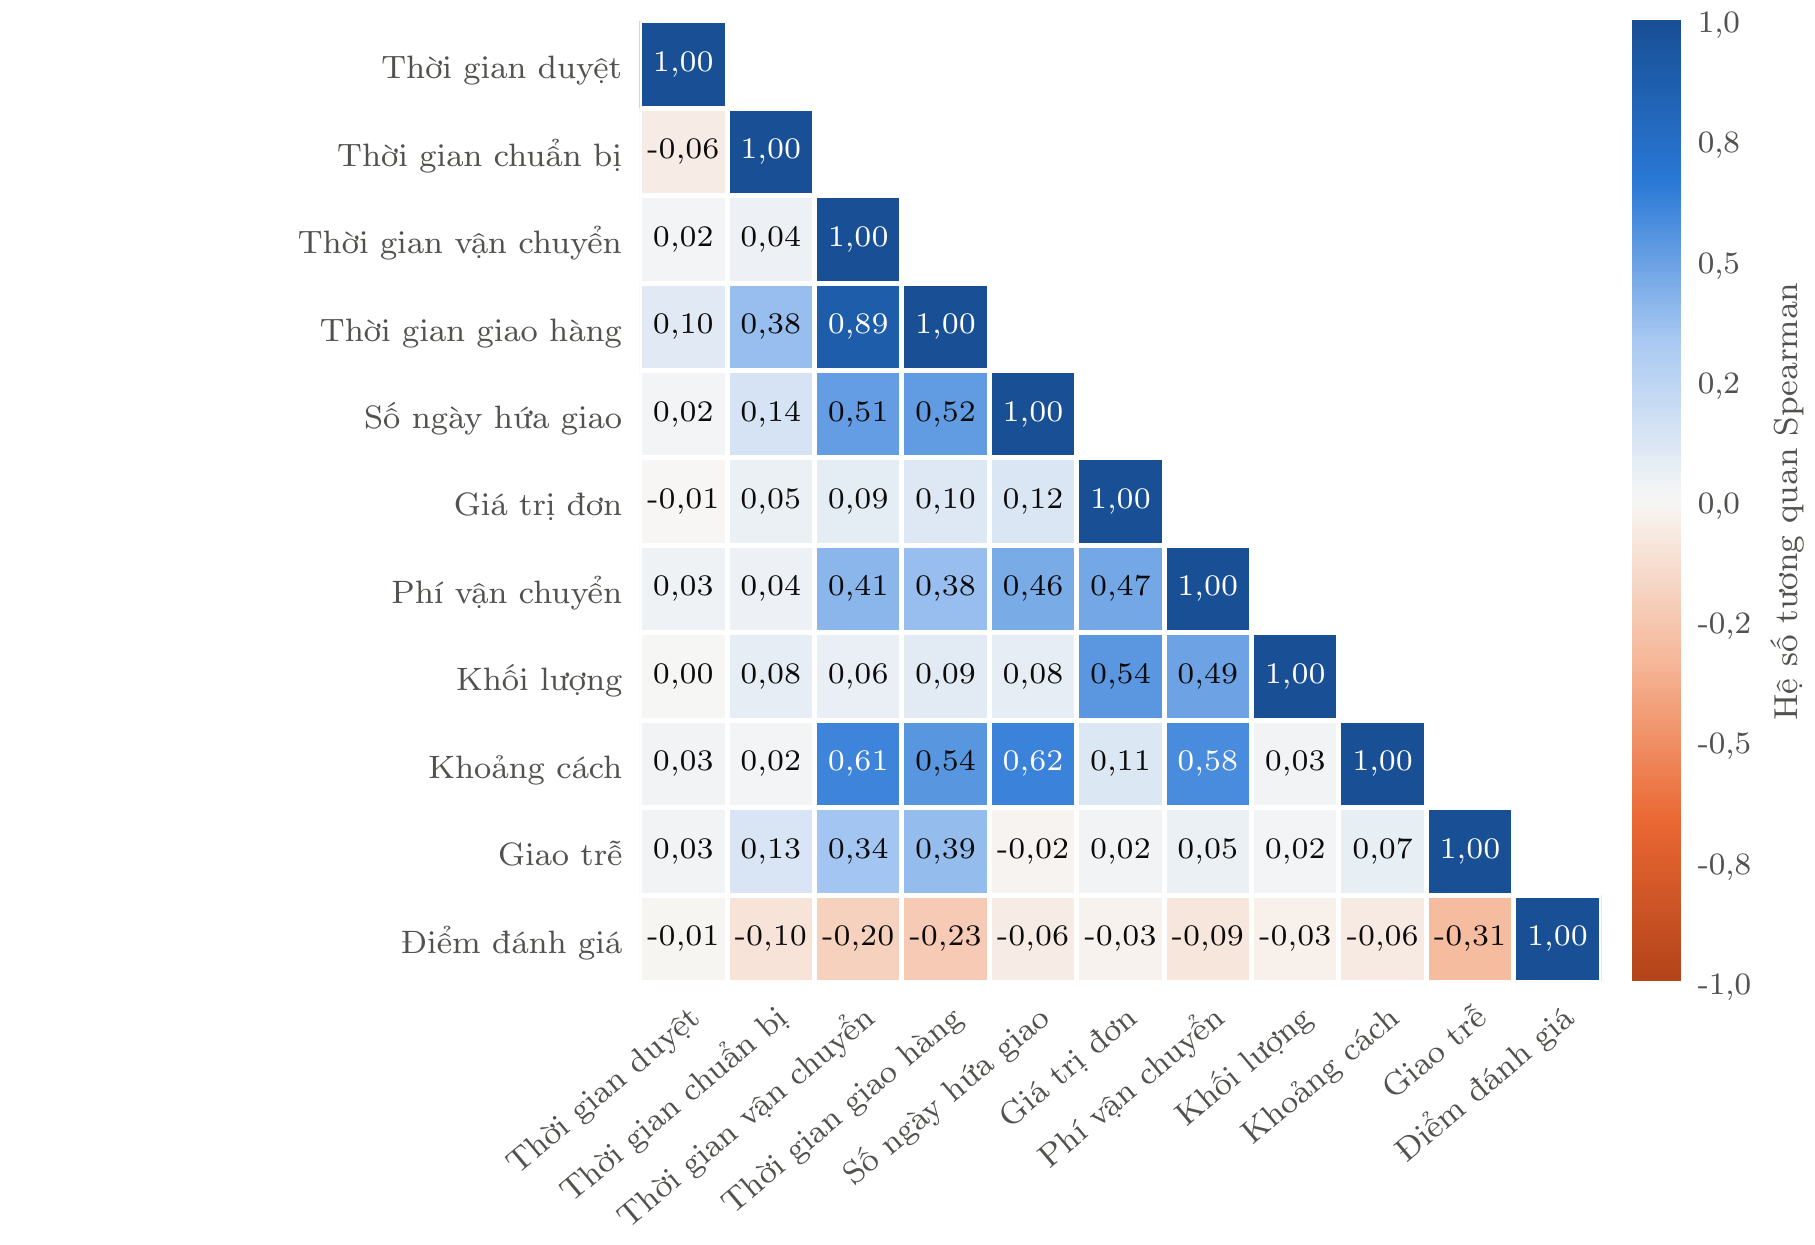
\includegraphics{Pictures/fig-eda-tuong-quan.png}
\caption{Ma trận tương quan Spearman giữa các thuộc tính ở mức đơn hàng (96.470 đơn đã giao)}
\label{fig:tuongquan}
\end{figure}

Ma trận cho thấy bốn điểm. Thứ nhất, điểm đánh giá tương quan mạnh nhất với cờ giao trễ ($-0{,}31$), mạnh hơn mọi thuộc tính về giá hay khối lượng; đây là dấu hiệu đầu tiên cho thấy giao trễ là vấn đề chính, và phần OLAP sẽ kiểm chứng điều này. Thứ hai, thời gian giao hàng gần như do thời gian vận chuyển quyết định (0,89), còn thời gian duyệt đơn hầu như không ảnh hưởng (0,10). Thứ ba, số ngày hứa giao tương quan khá chặt với khoảng cách (0,62) nhưng gần như không tương quan với giao trễ ($-0{,}02$): sàn đã cộng thêm ngày cho đơn đi xa, nên điều quyết định trễ hay không là ngày hứa có \textit{đủ dư} so với thời gian giao thường lệ hay không. Thứ tư, giá trị đơn, phí vận chuyển và khối lượng tương quan với nhau (0,47-0,54) nhưng không liên quan đến giao trễ.

\subsubsection{Tỷ lệ giao trễ theo nhóm giá trị}

Hệ số tương quan chỉ đo quan hệ đơn điệu, nên ba thuộc tính được chia thành các khoảng và tính tỷ lệ trễ của từng khoảng (Hình~\ref{fig:trenhom}). Tỷ lệ trễ tăng đều theo khoảng cách, từ 4,6\% với đơn dưới 100 km lên 12,0\% với đơn trên 2.000 km. Với số ngày hứa giao, quan hệ có dạng hình chuông: đơn được hứa 21-25 ngày trễ nhiều nhất (8,1\%), còn đơn hứa trên 30 ngày ít trễ nhất (5,0\%), đúng với nhận xét về độ dư ở trên. Rõ nhất là thời gian người bán chuẩn bị hàng: đơn được bàn giao trong vòng một ngày chỉ trễ 3,9\%, còn đơn mất hơn 10 ngày trễ tới 29,4\% và bị chấm trung bình 3,32 điểm.

\begin{figure}[H]
\centering
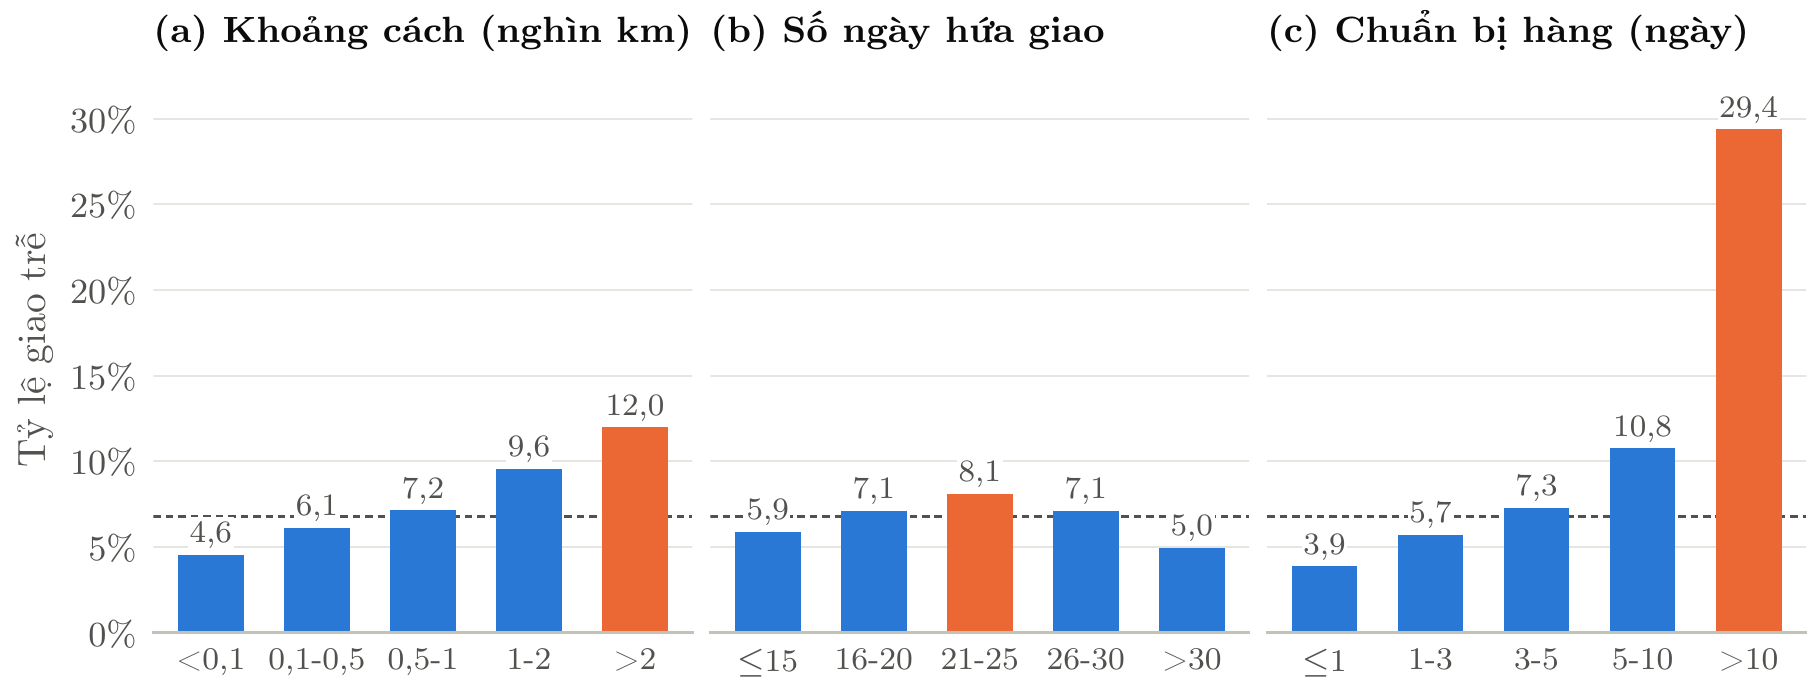
\includegraphics{Pictures/fig-eda-ty-le-tre-theo-nhom.png}
\caption{Tỷ lệ giao trễ theo khoảng cách giao (a), số ngày hứa giao (b) và thời gian người bán chuẩn bị hàng (c); đường đứt nét là tỷ lệ trễ chung 6,77\%}
\label{fig:trenhom}
\end{figure}

\subsubsection{Nhận xét}

Sau tiền xử lý, dữ liệu đã nhất quán: mỗi đơn có một trạng thái, một đánh giá, các mốc thời gian đúng thứ tự hoặc được để trống có lý do, và mọi khách hàng, người bán đều có thành phố, bang, vùng. Kết quả khám phá cũng định hướng cho các phần sau. Với kho dữ liệu, các thước đo về giao hàng và đánh giá phải tính ở mức đơn hàng, và cần chiều địa lý đủ chi tiết để phân tích theo tuyến giao. Với hệ hỗ trợ quyết định, thời gian chuẩn bị hàng, độ dư của ngày hứa giao và khoảng cách là những tín hiệu mạnh nhất về nguy cơ trễ; trong đó thời gian chuẩn bị hàng chỉ biết được khi người bán bàn giao cho đơn vị vận chuyển, nên đây là thời điểm hợp lý nhất để dự báo (mục~\ref{sec:dss}).
